\documentclass[a4paper,titlepage,twocolumn,oneside,12pt,ngerman,titlepage=firstiscover]{scrbook}
\usepackage{subfiles}
%for faster compiling - TODO remove in final version!
%\includeonly{minimizer_distribution/minimizer_distribution}
% Um während der Entwurfsphase weniger leere Seiten zu haben, kann man oben "twoside" durch "oneside" ersetzen.

\usepackage[english]{babel} % language
\usepackage[utf8]{inputenc} % encoding
\usepackage{amsmath,amsfonts,amssymb,amsthm} % mathematical expression, symbols, fonts, and the whole theorem environment engine
\usepackage{xcolor,graphicx} % graphics and colorings
\usepackage{tabularx,booktabs,multirow} % all about tables: booktabs gives the standard formatting, multirow allows cells to span over multiple rows.
%\usepackage{scrextend} % super powerful tool that helps a bit with everything
\usepackage[margin=0pt]{subcaption} % specific form for captions
\usepackage[autostyle]{csquotes} % helper for quoting

\usepackage{rotating} % if you want to rotate any object

\usepackage[backend=bibtex,
  style=alphabetic, % alphabetic ordered list
	hyperref=true, 
	natbib=true, % makes use of natbib
	backref=true, % additional writes for each bib-entry, on which pages its cites
	backrefstyle=three, % this style replaces e.g. 11,12,13 by 11-13
	sortcites=true, 
	maxbibnames=50,
	maxcitenames=3, % cites at most three authors---if more, only first author followed by et al. is written
 	firstinits=true, % nur Initialen anzeigen und auch nur nach diesen sortieren
% 	refsection=part,
% 	refsegment=chapter,
	isbn=false,url=true,doi=false] 
	{biblatex} % for references
	
% % if you want to change pageback references are stated, you can use the following:
% \DefineBibliographyStrings{english}{%
%   backrefpage = {see p\adddot},%
%   backrefpages = {see pp\adddot}%
% }

\bibliography{bibfile} % add the .bib file you use here

% please fill in the following data:
\newcommand{\mytitle}{Automatic Optimization of Level Parameters for RSHash}
\newcommand{\mysubtitle}{RSHash is a minimizer based fast, compressed hash table for storing DNA kmers. It was recently introduced by the Reinert Group.}
\newcommand{\myname}{Bjarne David Jehn}
\newcommand{\thesisType}{Bachelor's Thesis}

\usepackage[pdfdisplaydoctitle,menucolor=orange!40!black,filecolor=magenta!40!black,urlcolor=blue!40!black,linkcolor=red!40!black,citecolor=green!40!black,colorlinks]{hyperref}
\hypersetup{pdftitle={\mytitle}, pdfauthor={\myname}}

\usepackage{todonotes} % disable this package in final thesis!


%=========== Timestamp on each page. Helpful to keep track of versions. 
%=========== Remove in final thesis!!!
\usepackage{scalefnt}
\usepackage{scrtime}
\usepackage{eso-pic}
\AddToShipoutPicture{
	\put(20,50){\textcolor[gray]{0.5}{\begin{tabular}{l} \thesisType{} \hspace{1cm} \myname \\ \mytitle{} (Compile date: \today/\thistime)\end{tabular}}}
}
%=========== End Timestamp


%=========== graphics, in particular tikz
\usepackage{tikz}
\usetikzlibrary{arrows,decorations.pathmorphing,decorations.pathreplacing,backgrounds,positioning,fit,matrix}
\usetikzlibrary{shapes,calc,arrows.meta,positioning}

%=========== tables from csv files (helpful for experiments)
\usepackage{pgfplots}
\usepackage{siunitx}
\usepackage{pgfplotstable}

%=========== Pseudocode
\usepackage{algorithm}
\usepackage{algpseudocode}
\algnewcommand\algorithmicinput{\textbf{Input:}}
\algnewcommand\algorithmicoutput{\textbf{Output:}}
\algnewcommand\Input{\item[\algorithmicinput]}
\algnewcommand\Output{\item[\algorithmicoutput]}
\floatname{algorithm}{Algoritmus}

%=========== \cref is a powerfull command that automatically states the current environment (e.g. Theorem, Lemma, etc.)
\usepackage[sort&compress,nameinlink,noabbrev,capitalize]{cleveref}


%\usepgfplotslibrary{external}
%\tikzexternalize

%===========theorem environment
\theoremstyle{plain} % typical theorem-style (bold header, italic font)
\newtheorem{theorem}{Theorem}[chapter]
\newtheorem{lemma}[theorem]{Lemma}
\newtheorem{corollary}[theorem]{Korollar}
\newtheorem{observation}[theorem]{Beobachtung}
\newtheorem{proposition}[theorem]{Proposition}
\newtheorem{rrule}{Reduktionsregel}[section]

\crefname{rrule}{Reduktionsregel}{Reduktionsregeln} % how cleverref (\cref) has to handle these environments
\Crefname{rrule}{RR}{RRs} % with \Cref us can use what you defined here---somtimes useful if you want to abbreviate environment when citing (e.g. in tables or figures)

\theoremstyle{definition} % typical definition-style (bold header, normal font)
\newtheorem{definition}[theorem]{Definition}

\theoremstyle{remark} % typical theorem-style (italic header, normal font)
\newtheorem{example}{Example}
\newtheorem*{remark}{Remark}
\newtheorem{reduction}{Reduction}
\theoremstyle{plain}

%===========problem definition evironment: gets three arguments (1) problem name #1 (2) input specification #2 (3) question specification #3
\newcommand{\problemdef}[3]{
  \begin{center}
    \begin{minipage}{0.95\textwidth}
      \noindent
      \textsc{#1}
      
      \vspace{2pt}
      \setlength{\tabcolsep}{3pt}
      \begin{tabularx}{\textwidth}{@{}lX@{}}
        \textbf{Eingabe:} 		& #2 \\
        \textbf{Frage:} 	& #3
      \end{tabularx}
    \end{minipage}
  \end{center}
}



%=========== Nützliche Abkürzungen
\newcommand{\NN}{\mathbb{N}} % natürliche Zahlen
\newcommand{\RR}{\mathbb{R}} % reelle Zahlen
\newcommand{\QQ}{\mathbb{Q}} % rationale Zahlen
\newcommand{\ZZ}{\mathbb{Z}} % ganze Zahlen

\newcommand{\bigO}{\mathcal{O}} % Landausymbol

\newcommand\abs[1]{\left|#1\right|} % Betragsfunktion
\newcommand\norm[2]{\left\lVert#1\right\rVert_{#2}} % norm
\newcommand\enorm[1]{\norm{#1}{2}} % euclidean norm

%=========== commands for MINLP
\newcommand{\noam}{noam} %numberOfAppearingMinimizers

\newcommand{\lookupTime}{T_{lookup}}
\newcommand{\remainingTime}{T_{remaining}}

\newcommand{\timeForCheckInR}{{T_R}}
\newcommand{\timeForLookupInS}{{T_{SL}}}
\newcommand{\timeForHashtable}{{T_H}}

\newcommand{\percKmers}{\textbf{p}_\textbf{K}}
\newcommand{\percKmersEmpiric}{P_{K}}

\newcommand{\possibleMinimizerLength}{\mathcal{M}}
\newcommand{\possibleThresholds}{\mathcal{T}}

\newcommand{\minimizerLength}{\textbf{m}}
\newcommand{\threshold}{\textbf{t}}

\newcommand{\selectorm}{\mu}
\newcommand{\selectort}{\tau}

\newcommand{\levels}{\mathcal{L}}

\newcommand{\levelI}{{l}}
\newcommand{\levelOne}{1}
\newcommand{\levelTwo}{2}
\newcommand{\levelThree}{3}
%=========== commands for subsampling
\newcommand{\numberOfSamples}{n}
\newcommand{\lengthOfSamples}{l}

\newcommand{\genomeText}{T}
\newcommand{\sampledText}{T^S}

%========== Title Formating
\titlehead{
\begin{minipage}{0.8\textwidth}
\textbf{Technische Universität Berlin}\\
Faculty IV: Electrical Engineering and Computer Science\\
\textbf{Freie Universität Berlin}\\
Department of Mathematics and Computer Science\\
Algorithmic Bioinformatics\\
\todo[inline]{welche uni angeben, welche reihenfolge..?}
\end{minipage}
\hfill
\begin{minipage}{0.16\textwidth}

\includegraphics[width=\textwidth]{tu-logo}
\end{minipage}
\vspace{3.5cm}
}

\title{\mytitle}
\subtitle{(\mysubtitle)\vspace*{3cm}}

\author{
	\Large{\textbf{\thesisType{}}}\vspace{0.1cm}\\
	\textbf{\large{by \myname}}\vspace{0.1cm}\\
	\large{to obtain the degree of \grqq Bachelor of Science\grqq~(B. Sc.)}\\
	\large{in the Computer Science degree studies (Informatik)}
	\vspace*{3cm}\\
		\small{
			\begin{tabular}{rl}
			    First Reviewer:& Prof. Dr. Knut Reinert\\
			    \hspace{2cm}Second Reviewer:& Prof. Dr. Stephan Kreutzer\\
			    Supervisor:& Jonas Schulte-Mattler
			\end{tabular}
		}
	\vspace*{1cm}
}

\date{} % only month and year
\begin{document}

\selectlanguage{english}

\maketitle

\onecolumn
\section*{Declaration of Authorship}
\noindent
I hereby declare that the thesis submitted is my own, unaided work, completed without any external help. Only
the sources and resources listed were used. All passages taken from the sources and aids used, either
unchanged or paraphrased, have been marked as such.\\

Where generative AI tools were used, I have indicated the product name, manufacturer, the software version
used, as well as the respective purpose (e.g. checking and improving language in the texts, systematic
research). I am fully responsible for the selection, adoption, and all results of the AI-generated output I use.\\

I have taken note of the Principles for Ensuring Good Research Practice at TU Berlin dated 15 February 2023.
\url{https://www.static.tu.berlin/fileadmin/www/10002457/K3-AMBl/Amtsblatt\_2023/Amtliches\_Mitteilungsblatt\_Nr.\_16\_vom\_30.05.2023.pdf}\\

I further declare that I have not submitted the thesis in the same or similar form to any other examination
authority.\\

\begin{tabular}[h]{lll} Berlin, & \underline{\hspace{5cm}} & \underline{\hspace{7cm}}\\
 & \small{Date} & \small{Signature}
\end{tabular}
\normalsize
\twocolumn
\newpage

\section*{Abstract}

\newpage
\tableofcontents
\newpage


\documentclass[../thesis.tex]{subfiles}

\begin{document}
\chapter{MINLP Modeling}\label{chap:minlp}

\section*{One Level}
As a first approach we model the runtime and space consumption for only one level.\\
Let $\possibleMinimizerLength$ be the Set of all minimizer length and $\possibleThresholds$ the set of all thresholds to be considered.
\subsection*{Runtime}

\begin{table}
\caption{Constants and Variables for One Level}
\begin{tabularx}{\columnwidth}{|| l | X ||}
	\hline
	Constants	&  \\
	\hline
	$\timeForLookupInS$		& time to lookup a k-mer in vector S \\
	$\timeForHashtable$		& time to lookup a k-mer in the hash table \\
	$\percKmersEmpiric(m, t)$ &empirically estimated value for a k-mer with a minimizer \\
	& of length $m$ to have a frequency less than $t$ \\
	\hline
	\hline
	Variables	&  \\
	\hline
	$\percKmers \in \left[0,1\right]$ & probability of a k-mer to have a minimizer with frequency $\leq t$ \\
	$\selectorm_m \in \left\{0, 1\right\}$	& binary selector for every minimizer length $m \in \possibleMinimizerLength$\\
	$\selectort_t \in \left\{0, 1\right\}$	& binary selector for every threshold $t \in \possibleThresholds$\\
	\minimizerLength & optimal minimizer length\\
	\threshold & optimal threshold\\
	\hline 
\end{tabularx}
\end{table}

To lookup a k-mer $q$ with minimizer $m(q)$ of frequency $f(m(q))$ on one level, first the bit vector $R$ is checked in order to determin whether $1 \leq f(m) \leq threshold$. This can be ignored when modeling the lookup runtime as this is practically not influenced by the parameters. \todo{reason}\\
For $\percKmers$ of the k-mers, the corresponding bit in $R$ will be set, which results in a lookup in $S$. If $m(q)$ does not appear at all or has a $f(m(q)) > t$, a lookup in the hash table will follow. The lookup time $\lookupTime$ for one level can thus be modeled as:
\begin{equation*}
	\lookupTime = \timeForLookupInS * \percKmers + \timeForHashtable * (1-\percKmers)
\end{equation*}

In order to determine $m$ and $t$ we introduce binary selector variables $\selectorm_m$, $\selectort_t$ for each possible $m \in \possibleMinimizerLength$ and $t \in \possibleThresholds$.\\
$\selectorm_m$ should be $1$ exactly when the optimal minimizer length is $m$.\\
$\selectort_t$ should be $1$ exactly when the optimal threshold is $t$.\\
The selectors for $m$ and $t$ must be binary and mutually exclusive:
\begin{align*}
	&\selectorm_m \in {0,1} \mid \forall m \in \possibleMinimizerLength \\
	&\selectort_t \in {0,1} \mid \forall t \in \possibleThresholds \\
	&\sum_{m \in \possibleMinimizerLength} \selectorm_m = 1 \\
	&\sum_{t \in \possibleThresholds} \selectort_t = 1
\end{align*}

For a fixed minimizer length $m$ and threshold $t$ let $\percKmersEmpiric(m, t)$ be the empirically determined percentage of k-mers $q$ that have a minimizer with $f(m(q)) < t$.\\
We can then model $\percKmers$ with:
\[ \percKmers = \sum_{m \in \possibleMinimizerLength} \left( \selectorm_m \sum_{t \in \possibleThresholds} \percKmersEmpiric(m, t) * \selectort_t\right) \]
$\minimizerLength$ and $\threshold$ can then be determined by:
\begin{align*}
	\minimizerLength &= \sum_{m \in \possibleMinimizerLength} \selectorm_m * m \\
	\threshold &= \sum_{t \in \possibleThresholds} \selectort_t * t
\end{align*}
\\
The above results in the following MINLP (Mixed Integer Non Linear Program):\\
\\
MINIMIZE
\begin{align*}
	\lookupTime = \timeForLookupInS^\levelOne * \percKmers + \timeForHashtable * (1-\percKmers)
\end{align*}
SUBJECT TO
\begin{align*}
		&\percKmers = \sum_{m \in \possibleMinimizerLength} \left( \selectorm_m \sum_{t \in \possibleThresholds} \percKmersEmpiric(m, t) * \selectort_t\right)\\
		&\selectorm_m \in {0,1} \mid \forall m \in M \\
		&\selectort_t \in {0,1} \mid \forall t \in T \\
		&\sum_{m \in M} \selectorm_m = 1 \\
		&\sum_{t \in T} \selectort_t = 1 \\
		&\minimizerLength = \sum_{m \in \possibleMinimizerLength} \selectorm_m * m \\
		&\threshold = \sum_{t \in \possibleThresholds} \selectort_t * t
\end{align*}
\\
For now we will assume that $\timeForLookupInS \approx 40ns$ and $\timeForHashtable \approx 20ns$.\\
Solving this MINLP will result in a Solution where the $\selectorm_m$, $\selectort_t$ corresponding to the smallest $m \in \possibleMinimizerLength$, $t \in \possibleThresholds$ will be set to one.\\
This is as expected, since this leads to the smallest possible $\percKmers$. This minimizes the k-mers found in the vector $S$ and thus maximizes the lookups in the (faster) hash table.\\
\\
However this also results in a high space consumption, because each entry in the hash table containing the minimizer as a key and the offset as its value is significantly larger than an entry in $S$ which only contains offsets.\\
\\
In order to take that into account, we have to add a constraint modeling the space consumption.\\

\subsection*{Space Consumption}
The space consumption of the Data Structure used by RSHash can be split into that of the Vectors $R$, $O$ and $S$ as well as the hash table $H$.

\subsubsection*{Bit Vectors $R$ and $S$}
$R$ and $S$ can likely be disregarded when modeling the space consumption. \todo{explain why}\\
$R$ is a Bit Vector of length $4^\minimizerLength$ that contains $n$ \todo{possibly model n?} 1s marking the existence of each encountered minimizer. Using Elias-Fano-Encoding, its size can be compressed to
\[ n \rceil log(4^\minimizerLength/n) \rceil + 3n\]

\subsubsection*{Offsetvector $O$}
$O$ contains one entry of size $log |T|$ for the offset of every minimizer with frequency $\leq t$ in $T$.\\
Every minimizer of length $\minimizerLength$ covers an average of $\frac{k-\minimizerLength+2}{2}$ consecutive k-mers. We can thus model the bits per k-mer in $O$ as:\\
\[bpk_O = \percKmers * \frac{2}{k-\minimizerLength+2} * log |T| \]

\subsubsection*{Hash table $H$}
For $1-\percKmers$ of the k-mers $q$ in $T$ $H$ contains an entry $(key:q, value:offset(q))$\\
Each entry has size $size(key) + size(value) = 64 + log |T|$.\\
The bits per k-mer required for the hash table can thus be modeled by
\[ bpk_H = (1-\percKmers) * (64 + log|T|)\]
%However $H$ also contains a number of empty buckets requiring the same amount of space. \todo{reason}\\
%For a hash table with $b$ buckets containing $n$ elements, the load factor $\alpha$ is defined as:
%\[\alpha = \frac{n}{b}\].\\
%That means that for every entry in the hash table, there must be $\frac{1-\alpha}{\alpha}$ many empty buckets.\\
%Using this we can model the bits per k-mer in $H$ as:\\
%\[bpk_H = (\alpha + \frac{1-\alpha}{\alpha}) * \frac{2}{k-\minimizerLength+2} * (1-\percKmers) * log |T| \]

\section*{Several Levels}
Let
\begin{table}
	\caption{Constants and Variables for Several Level}
	\begin{tabularx}{\columnwidth}{|| l | X ||}
		\hline
		Constants	&  \\
		\hline
		$\timeForLookupInS$		& time to lookup a k-mer in vector S\\
		$\timeForHashtable$		& time to lookup a k-mer in the hash table \\
		$\percKmersEmpiric(m, t)$ &empirically estimated value for a k-mer with a minimizer \\
		& of length $m$ to have a frequency less than $t$ \\
		\hline
		\hline
		Variables	&  \\
		\hline
		$\percKmers^l \in \left[0,1\right]$ & probability of a k-mer to have a minimizer with frequency $\leq t$ on level $l$ \\
		$\selectorm_m^l \in \left\{0, 1\right\}$	& binary selector for every minimizer length $m \in \possibleMinimizerLength$ on level $l$\\
		$\selectort_t^l \in \left\{0, 1\right\}$	& binary selector for every threshold $t \in \possibleThresholds$ on level $l$\\
		$\minimizerLength^l$ & optimal minimizer length on level $l$\\
		$\threshold^l$ & optimal threshold on level $l$\\
		\hline 
	\end{tabularx}\\
\end{table}
\subsection*{Runtime}
RSHash uses several levels, to make use of the skewniss of minimizer distribution.\\
Each level $l$ has a pair of parameters $\minimizerLength^l, \threshold^l$ which result in a probability $\percKmers^l$ of a k-mer belonging to level $l$.\\
For now, we still assume, that the time for a lookup in the vectors $R,S$ as well as the hash table $H$ are (practically) independent of the parameters $\minimizerLength^l, \threshold^l$. \todo{reason}\\
\\
When using $L$ levels, the probability of a k-mer belonging to a higher level is dependent on the probability of k-mers belonging to the levels below.\\
On each level $1 \leq l \leq L$, for $\percKmers^l$ of the k-mers, the lookup will be completed by finding a value in the offset vector on that level whilst the remaining $(1-\percKmers^l)$ queries result in a lookup on the next level.\\
We can model the lookup time for all levels $1\leq l<L$ levels recursively as:
\[ 
\lookupTime^l =
\begin{cases}
	\percKmers^l*\timeForLookupInS + (1-\percKmers^l)*\lookupTime^{l+1} &\mid 1\leq l \leq L\\
	\timeForHashtable &\mid l=L+1
\end{cases}
\]
For $L=3$ levels, this results in:
\[
\begin{array}{llll}
	\lookupTime =
	&\percKmers^\levelOne*\timeForLookupInS\\
	&+ (1-\percKmers^\levelOne) * \Bigg(&\percKmers^\levelTwo*\timeForLookupInS\\
			&&+(1-\percKmers^\levelTwo) * \Big( &+ \percKmers^\levelThree*\timeForLookupInS\\
				&&&+ (1-\percKmers^\levelThree) * \timeForHashtable \Big) \Bigg)
\end{array}
\]

Because $\minimizerLength^l$ and $\threshold^l$ can be different on every level $l$, a different set of binary selector variables $\selectorm^l_m$ and $\selectort^l$ is needed.\\
The constraints for each level are the same as for one level:
\[ \begin{array}{ll}
	\selectorm_m^l \in {0,1} & \mid \forall (l,m) \in (\levels \times \possibleMinimizerLength) \\
	\selectort_t^l \in {0,1} & \mid \forall (l,t) \in (\levels \times \threshold) \\
	\sum_{m \in \possibleMinimizerLength} \selectorm_m^l = 1 & \mid \forall l \\
	\sum_{t \in \possibleThresholds} \selectort_t^l = 1 & \mid \forall l
\end{array} \]

For every level $l$ $\percKmers^l, \minimizerLength^l$ and $\threshold^l$ can also be modeled analogously to having only one level: \todo{this only holds under the assumption, that the minimizer distribution is equal on each level - independent of the choice of m and t. This is not trivial and should be further explored!!}
\begin{align*}
	\percKmers^l &= \sum_{m \in \possibleMinimizerLength} \left( \selectorm_m^l \sum_{t \in \possibleThresholds} \percKmersEmpiric(m, t) * \selectort_t^l\right) & \mid \forall l \in \levels\\
	\minimizerLength^l &= \sum_{m \in \possibleMinimizerLength} \selectorm_m^l * m  & \mid \forall l \in \levels\\
	\threshold^l &= \sum_{t \in \possibleThresholds} \selectort_t^l * t & \mid \forall l \in \levels
\end{align*}


\subsection*{Space Consumption}
\subsubsection*{Offsetvector $O$}
For several levels, the offset vector for level $l$ only contains an entry for a k-mer $q$, if the k-mers minimizer $m(q)$ has a frequency $f(m(q)) > t^{i}$ for all levels $1 \leq i < l$ and $f(m(q)) \leq t^{l}$. \todo{should I introduce an index for the minimizer function as it differs for every level? e.g. $m^l(q)$}\\
The bits per k-mer for the Offset vector on level $l$ can thus be modeled as:
\[bpk_{O^l} = \prod_{i=1}^{l-1} (1-\percKmers^i) * \percKmers^l * \frac{2}{k-\minimizerLength^l+2} * log |T| \]

\subsubsection*{Hash table $H$}
The hash table only contains an entry k-mers $q$, for which $f(m(q)) > t^l$ for all levels $1 \leq l \leq L$.\\
The bits per k-mer for the hash table can thus be modeled as 
\[ bpk_H = \prod_{l=1}^{L} (1-\percKmers^l) * (64 + log|T|)\]

\section*{Limitations}
This approach of solving the constructed model has the advantage (\todo{over what}) of finding optimal results \todo{does it?}.\\
However for large genomes, finding the empirical values $\percKmersEmpiric(m,t)$ becomes increasingly time consuming and needs a lot of RAM \todo{how much, why?}.\\
\todo[inline]{paragraph/section about the complexity of finding the solution}

For these reasons, an approach yielding a solution that is a certain approximation of the optimum but takes less time to find it could be of interest.\\
An easy adaption  to speed up the search for empirical values would be to only sample part of the genome. By sampling sequences of length \todo{what length} at a large \todo{how lorge} number of random locations, the probability of choosing a bad representation becomes highly unlikely.\\
By sampling only part of the genome, we can speed up the finding of empirical values by a factor of \todo{factor} / or even "get it down to a constant" (that is for a fixed number of sample locations - regardless of the genomes size. this however results in a growing error for larger genomes).\\



\end{document}

\chapter{Minimizer Distribution}
The \nameref{chap:minlp} only works, if the values $\percKmers(m,t)$ are known for every $(m,t) \in \possibleMinimizerLength \times \possibleThresholds$ for the input sequence.
\section*{Determining the Distribution}
The code to find the minimizer distribution for a given $sequence, k, \minimizerLength$ and $\threshold$ follows the following steps:\\
stats:\\
\begin{enumerate}
	\item $count_minimizers$:
		\begin{enumerate}
			\item set $kmers \leftarrow |sequence|-k+1$
			\item parse every kmer in the $sequence$ and add all minimizers to a vector $minimizers$ \todo{Zeile 48-55: verstehe ich es richtig, dass in der schleife in Zeile 52 jeder minimizer nur einmal zum vektor hinzugefügt wird, auch wenn er mehrere kmere abdeckt?}
			\item sort $minimizers$
			\item iterate over the sorted vector and
			\begin{itemize}
				\item count the occurences of each minimizer
				\item add all unfrequent minimizers to a new vector $unfrq_minimizers$
				\item store their occurences in the vector $counts$ where $counts[i]$ relates to $unfreq_minimizers[i]$
				\item store the sum of all occurences in $no_skmers$
			\end{itemize}
		\end{enumerate}
	\item $minimizers \leftarrow unfreq_minimizers$
	\item $no_minimizers \leftarrow |minimizers|$
	\item $r \leftarrow$ elias-fano-compressed bitvector of length $2^{2\minimizerLength}$ that contains 1s at those positions $i$, for which the minimizer of value $i$ is present in $minimizers$
	\item $s \leftarrow$ corresponding vector $S$
	\item weiter ab Zeile 161
\end{enumerate}


\chapter{Subsampling}
\section*{Motivation}
The time for processing a genome in order to find the minimizer distribution $\percKmers(m,t)$ for possible minimizer lengths $m \in \possibleMinimizerLength$ and thresholds $t \in \possibleThresholds$ is directly proportional to the size of the genome.\\
For large genomes, this processing can become the dominating factor when searching for optimal parameters using the \nameref{chap:minlp} approach. In order to speed up the search for the empirical values, we introduce a subsampling method.

\section*{Subsampling Method}
Instead of calculating the distribution over the full genome, we sample $\numberOfSamples$ sequences of length $\lengthOfSamples \geq k$ at random positions in the genome.\\
\todo[inline]{how to handle overlapping samples}

\section*{Time Complexity of Finding the Minimizer Distributions}
\todo[inline]{genaue zeitliche abhängigkeit 1. verstehen und 2. aufschreiben}

\section*{Time Complexity using Subsampling}
By applying the proposed subsampling strategy, the original genome $\genomeText$ of length $|\genomeText|$ is reduced to the subsampled text $\sampledText$ of length $|\sampledText| = \numberOfSamples * \lengthOfSamples$. This means a reduction in size by a factor of $\frac{|\genomeText|}{|\sampledText|}$.\todo{assuming no overlaps}\\
Depending on the choice of $\numberOfSamples$ and $\lengthOfSamples$ this results in a speedup of the processing time by a factor of $ $\todo{factor} or even a constant processing time $ $\todo{time} when both parameters are chosen as a constand regardless of $|\genomeText|$ (this however should result in a growing error for larger genomes).

\section*{Error Analysis}

\section*{Choosing $\lengthOfSamples$}
The length $\lengthOfSamples$ has to be at least $k$. 
\todo[inline]{wenn $l > k$ ist, überlappen sich mehrere kmere an den gesampleten stellen. ich verstehe noch nicht, warum genau dass von vorteil ist.\\ Ist es für die Konstruktion der Burrow-Wheeler-Transformation relevant, bze. findet diese hier überhaupt statt?\\ oder lässt sich ein streaming case für ministats implementieren/ ist dies bereits so umgesetzt?}

\section*{Choosing $\numberOfSamples$}
Choosing a constant $\numberOfSamples$ would result in a processing time that would no longer be dependent of the genomes length $|\genomeText|$, as the sampled text would have constant size $\numberOfSamples * \lengthOfSamples$\todo{assuming no overlaps}. For large genomes, the percentage $\frac{|\sampledText|}{|\genomeText|}$ of the genome represented in the subsample can become arbitrarily small, resulting in growing error.\\
If instead $\numberOfSamples$ is chosen relative to $|\genomeText|$, $\frac{|\sampledText|}{|\genomeText|}$ will have a constant value independent of the genomes size. Even though this means, that the time needed, in order to find the minimizer distributions would still be proportional to the genomes size, this should be the preferred option as it results in a bounded error of the approximation.
\\
For a large enough $\numberOfSamples$, the probability of choosing a bad representation becomes highly unlikely.\todo{zu vage, begründen}\\

%\chapter{Introduction}\label{chap:introduction}

%wofür das alles?
\newcommand{\vehiclecaps}{B}
\newcommand{\vehiclecap}{\beta}
\newcommand{\vehicetype}{v}
\newcommand{\soc}{q}
\newcommand{\places}{\mathcal{X}}
\newcommand{\depot}{\delta}
\newcommand{\depots}{D}
\newcommand{\trips}{\mathcal{T}}
\newcommand{\trip}{\tau}
\newcommand{\chargers}{\mathcal{C}}
\newcommand{\charges}{Z}
\newcommand{\timefunc}{T}
\newcommand{\energyfunc}{Q}
\newcommand{\numbervt}{m}
\newcommand{\chargefunc}{Q^C}
\newcommand{\charge}{\zeta}
\newcommand{\vehicleschedule}{\psi}
\newcommand{\schedule}{\Psi}
\newcommand{\evehicleschedule}{\omega}
\newcommand{\eschedule}{\Omega}
\newcommand{\departure}{d}
\newcommand{\arrival}{a}
\newcommand{\timestart}{s}
\newcommand{\timeend}{e}
\newcommand{\chargestation}{c}
\newcommand{\vehicletypes}{\mathcal{V}}




\section{Motivation}\label{sec:motivation}

Laut \citet{Nie06} ist unser Thema voll wichtig.

\section{Stand der Forschung}

Mehrere Zitate auf einmal: \citet{Nie06,GJ79,KN12}

\chapter{Notation und Grundlegendes}\label{ch:notation}
Die Arbeit sollte so gut wie möglich alle zum Verständnis notwendinge Definition, Notation, Konventionen beinhalten.
Dieser Abschnitt ist dafür geeignet.

\paragraph*{Graphentheorie.} 
Sei~$G=(V,E)$ ein ungerichteter Graph, wobei~$V$ die Knotenmenge und~$E\subseteq \{\{v,w\}\mid v,w\in V,\, v\neq w\}$ die Kantenmenge bezeichnen.
Für einen Graphen~$G$ schreiben wir auch~$V(G)$ und~$E(G)$ für die Knoten- beziehungsweise Kantenmenge von~$G$.

Wenn man viel Notation einzuführen hat, dann kann ein sogenanntes \emph{labeling} empfehlenswert sein.
Wir nennen
\begin{labeling}{$\deg^i_G(v)$}
	\item[$V(G)$] die \emph{Knotenmenge} von~$G$;
	\item[$E(G)$] die \emph{Kantenmenge} von~$G$ mit~$E(G) \subseteq \binom{V(G)}{2}$; die Knoten~$u$ und~$v$ einer Kante~$e = \{u, v\} \in E(G)$ werden \emph{Endpunkte} genannt;
	\item[$n_G$] die Anzahl~$|V(G)|$ der Knoten;
	\item[$m_G$] die Anzahl~$|E(G)|$ der Kanten.
\end{labeling}

\paragraph*{Parametrisierte Komplexität.} 
Wir verwenden Standardnotation aus der Parametrisierten Komplexität und Algorithmik~\cite{Nie06}.

\chapter{\LaTeX{}-Beispiele}

\section{Grundlegendes}
Einzelne Zeilenumbrüche
sind 
Latex egal.
Mit einem doppelten Umbruch

erzeugt man einen neuen Absatz.
Der Übersicht halber sollte man die Zeilen im Latex-Quellcode trotzdem nicht zu lang machen.

Mit newcommand lassen sich eigene Befehle definieren:
\newcommand{\sfe}{supercalifragilisticexpialigetisch}
Jede \sfe{}e Instanz lässt sich mit einem \sfe{}en Algorithmis in \sfe{}er Zeit lösen.
(Sehr nützlich, wenn man später Dinge umbenennen will.)

\section{Formatierung}
\textit{Ich bin kursiv}.
\textbf{Ich bin fett}.
\textsc{Ich bin in Kapitälchen} (für Problemnamen).
\enquote{Ich stehe in Anführungszeichen.}

Hier kommt eine Formel: $a = b + c$.
Die nächste Formel kriegt mehr Platz und wird am \&-Zeichen ausgerichtet:\footnote{Man kann auch an mehreren Stellen ausrichten.}
\begin{align*}
	f : \RR &\to \RR \\
	x &\mapsto x^2
\end{align*}

Ohne Sternchen gibt's Zeilennummern:
\begin{align}
	a &= \abs{x - 2}\\
	b &= \enorm{a + x}\\
	c &= a^2 + b^2 \\
	\sqrt{17} &> 1 \label{eq:wurzel}
\end{align}

Hoch- und tiefgestellt wird so: $x_1, x^2, x_{i,j}^t$

Brüche schreibt man $\frac{n!}{k!(n-k)!}$ oder im Fließtext auch einfach $n!/(k!(n-k)!)$.

Ein paar weitere Operatoren:
\begin{align*}
	\sum_{i=1}^n \int_a^b \lim_{x \to \infty} \max_{y \geq x} \left\{ x \cdot y \middle| \left[ x^2 - y^2 \right] \subseteq \tilde{\Omega} \right\}
\end{align*}

Nützliche Buchstaben: $\ell, \theta, \vartheta, \epsilon, \varepsilon, \phi, \varphi$

Nützliche Relationen: $G \neq H \simeq K \cong T \approx \emptyset$.

Wer den Namen für ein bestimmtes Symbol sucht schaut am besten auf \url{http://detexify.kirelabs.org/}

Wenn man Text innerhalb einer Formel einfügen möchte, muss dieser mit \textit{\textbackslash text} ausgezeichnet werden:
\begin{align*}
	V &= \frac{4}{3} \pi z^3 & \text{Volumen einer Kugel mit Radius $z$}\\
	V &= \pi z^2 a = \pi zza & \text{Volumen einer Pizza mit Radius $z$ und Dicke $a$}
\end{align*}

Versuche Zeilenumbrüche an mathematischen Ausdrücken wie den nun hier folgenden $G$ zu vermeiden. 
Verwende die Tilde im Latex-Code um das zu vermeiden, wie folgt.

Versuche Zeilenumbrüche an mathematischen Ausdrücken wie den nun hier folgenden~$G$ zu vermeiden. 

Und noch was: Sätze sollten auch nicht mit mathematischen Ausdrücken beginnen.
Also, statt \enquote{$G$ ist toll.} besser \enquote{Graph~$G$ ist toll.}.


\section{Theoreme \& Co}


\begin{definition}\label{def:smaller}
	Für $a, b \in \RR$ schreiben wir $a < b$ falls gilt
	\todo[inline]{hier feht noch was. Manchmal ist es sinnvoll etwas lokal statt in \cref{ch:notation} zu definieren.}
\end{definition}

\begin{lemma}[trivial]\label{thm:trivial}
	$a < b \iff b > a$
\end{lemma}
\begin{proof}
	Gilt nach \cref{def:smaller}.
\end{proof}

\begin{theorem}[Robertson, Seymour]
	Die Menge der endlichen Graphen ist wohlquasigeordnet bzgl. der Relation \enquote{$\preceq$}.
\end{theorem}
\begin{proof}
	Folgt aus \cref{thm:trivial} in Verbindung mit \cref{eq:wurzel} (Übungsaufgabe).
\end{proof}

\newcommand{\vertexcover}{\textsc{Vertex Cover}}
\problemdef{\vertexcover{}}
{Ein Graph $G$, $k \in \NN$.}
{$\exists C \subseteq V(G) : \abs{C} = k$ und $\forall e \in E(G): e \cap C \neq \emptyset$?}

\begin{observation}\label{thm:exponentialzeit}
	\textsc{\vertexcover{}} ist lösbar in exponentieller Zeit.
\end{observation}

Aus \cref{thm:exponentialzeit} folgt unmittelbar das folgende \cref{thm:entscheidbar}.

\begin{corollary}\label{thm:entscheidbar}
	\textsc{\vertexcover{}} ist entscheidbar.
\end{corollary}

\begin{example}
	Ein interessantes Beispiel.
\end{example}

\begin{remark}
	Eine Anmerkung.
\end{remark}


\section{Abbildungen}

Beispiele für Graphen sind in \cref{fig:graph} abgebildet.
Hierbei ist \cref{fig:directed_graph} ein \textit{gerichteter Graph} (auch \textit{Digraph}).

Wer zu faul ist, die Bilder in tikz zu erstellen, kann sich auch \url{http://ipe.otfried.org/} anschauen.

\begin{figure}[t]
	\centering
	\tikzstyle{alter}=[circle, minimum size=16pt, draw, inner sep=1pt] 
	\tikzstyle{majarr}=[draw=black]
	\begin{subfigure}[t]{.45\textwidth}
		\centering
		\begin{tikzpicture}[auto, >=stealth',shorten <=1pt, shorten >=1pt]
			\node[alter] at (0,0) (a) {$a$};
			\node[alter, right = 8ex of a] (b) {$b$};
			\node[alter, right = 8ex of b] (c) {$c$};
			
			\draw[majarr] (a) edge (b);
			\draw[majarr] (b) edge (c);
			\draw[majarr] (a)[bend left=43] edge (c);
		\end{tikzpicture}
		\caption{ungerichtet}
		\label{fig:undirected_graph}
	\end{subfigure}  
	\begin{subfigure}[t]{.45\textwidth}
		\centering
		\begin{tikzpicture}[auto, >=stealth']
			\tikzstyle{majarr}=[draw=black,->,shorten <=1.5pt, shorten >=1.5pt]
			\node[alter] at (0,0) (a) {$a$};
			\node[alter, right = 8ex of a] (b) {$b$};
			\node[alter, right = 8ex of b] (c) {$c$};
			
			\draw[majarr] (a) edge node[midway, anchor=south] {$\scriptstyle 1$} (b);
			\draw[majarr] (b) edge node[midway, anchor=south] {$\scriptstyle 2$} (c);
			\draw[majarr] (a) edge[bend left=43] node[midway, anchor=south] {$\scriptstyle 3$} (c);
		\end{tikzpicture}
		\caption{gerichtet}
		\label{fig:directed_graph}
	\end{subfigure}
	\caption{Beispiele für Graphen. Achtung: \textit{label} immer \textbf{nach} \textit{caption}, sonst gehen die Verweise kaputt.}
	\label{fig:graph}
\end{figure}



\Cref{tab:some-table} ist eine große Tabelle.
Normalerweise versucht Latex selbst, einen geeigneten Ort für Abbildungen zu finden.

Externe Bilder lassen sich auch einbinden (siehe \cref{fig:comic}).

\begin{table}[t]
	\caption{\normalfont
		Ergebnisse der Laufzeitexperimente. Alle Zeiten sind in Sekunden angegeben.
		Im Gegensatz zu Abbildungen, Tabellenüberschriften sind über der Tabelle zu platzieren.
	}
	\centering
	\footnotesize
	\renewcommand{\tabcolsep}{7pt}
	\begin{tabular}{ll rr rrr}
		\toprule
		&	file 				& $n$ 		& $m$  		& \texttt{WCC} [s]&\texttt{HKN} [s]	& \texttt{CHLS} [s] \\
		\midrule
		\multirow{4}{*}{\rotatebox[origin=c]{90}{Clustering}} 
		& email 				& 1K	 	& 5K	 	& 0.67 		& 48.75 		& 2.51 	 \\
		& hep-th 				& 7K	 	& 15K	 	& 0.43 		& 1.35 			& 3.75 	 \\
		& netscience 			& 1K	 	& 2K	 	& 0.24 		& 0.37 			& 0.07 	 \\
		& PGPgiantcompo 		& 10K	 	& 24K	 	& 0.67 		& 1.70 			& 3.51 	 \\
		\midrule
		\multirow{4}{*}{\rotatebox[origin=c]{90}{Co-author}} 
		& citationCiteseer 		& 268K	 	& 1.1M		& 21.46 	& 83.90 		& --- 	 \\
		& coAuthorsCiteseer 	& 227K	 	& 0.8M	 	& 11.46 	& 50.35 		& --- 	 \\
		& coAuthorsDBLP 		& 289K	 	& 0.9M		& 15.76 	& 78.51 		& --- 	 \\
		& coPapersCiteseer 		& 434K	 	& 16M		& ---		& ---			& --- 	 \\
		\bottomrule
	\end{tabular}
	\label{tab:some-table}
\end{table}

\begin{figure}
	\centering
	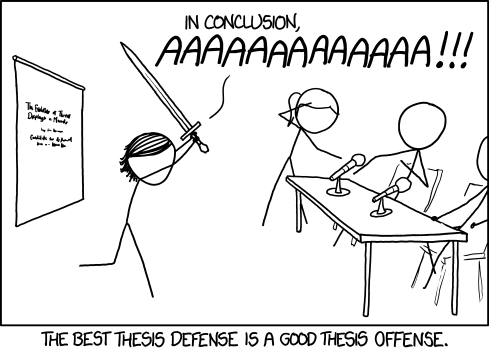
\includegraphics[scale=0.7]{figures/thesis_defense.png}
	\caption{MY RESULTS ARE A SIGNIFICANT IMPROVEMENT ON THE STATE OF THE AAAAAAAAAAAART \cite{xkcd1403}}
	\label{fig:comic}
\end{figure}


\pgfplotstableread[col sep = comma]{example-data.csv}\data % read the csv-file
\begin{table}
	\small
	\caption{\normalfont Bonustabelle (automatisch generiert aus example-data.csv) Die Beschriftung ist immer über Tabellen aber unter Bildern...}
	\pgfplotstabletypeset[columns={graphname,vertices,edges, mmtime,kerneltime,kernelvertices,kerneledges,kmmtime},
	columns/graphname/.style={string type,column name=Graph,column type = {r}},
	columns/vertices/.style={column name=$n$,precision=1,column type = {r}},
	columns/edges/.style={column name=$m$,precision=1,column type = {r}},
	columns/mmtime/.style={column name=blossom5,fixed,precision=2,dec sep align,preproc/expr={0.001*##1 + 0.01}},
	columns/kerneltime/.style={column name=kernel,fixed,precision=2,dec sep align,preproc/expr={0.001*##1 + 0.01}},
	columns/kernelvertices/.style={column name=$n'$,precision=1,column type = {r}},
	columns/kerneledges/.style={column name=$m'$,precision=1,column type = {r}},
	columns/kmmtime/.style={column name=blossom5',precision=2,fixed,dec sep align,preproc/expr={0.001*##1 + 0.01}},
	every head row/.style ={before row=\toprule, after row=\midrule},
	every last row/.style ={after row=\bottomrule}]{\data}
\end{table}


\section{Pseudocode}

\Cref{alg:euclid} ist Euklids Algorithmus zur Bestimmung des größten gemeinsamen Teilers zweier Zahlen.
Die Schleife in \cref{line:loop} terminiert sobald $a$ durch $b$ teilbar ist.

Für mehr Informationen zu Pseudocode in \LaTeX, empfiehlt sich ein Blick in die algorithmicx-Anleitung \cite{algorithmicx}.



\begin{algorithm}
	\caption{Euklids Algorithmus}\label{alg:euclid}
	\begin{algorithmic}[1]
		\Input{$a, b \in \NN$}
		\Output{Der größte gemeinsame Teiler von $a, b$}
		\Function{Euklid}{$a,b$}
		\State $r\gets a\bmod b$ \Comment{$r$ ist der Rest der Ganzzahl-Division $a / b$}
		\While{$r\not=0$} \label{line:loop}
		\State $a\gets b$
		\State $b\gets r$
		\State $r\gets a\bmod b$
		\EndWhile
		\State \textbf{return} $b$
		\EndFunction
	\end{algorithmic}
\end{algorithm}


\chapter{Conclusion}

Ein Fazit is keine Zusammenfassung.
Grob sollten hier erzielte Ergebnisse diskutiert und ein Ausblick für weitere Forschung gegeben werden.

Wir habe dieses tolle Ergebnis.
Allerdings blieb diese andere tolle Frage offen.
Wir vermuten, dass die Frage positive zu beantworten ist wegen diesem tollen Argument.

\printbibliography[heading=bibintoc,title={Literatur}]

\end{document}
